\section{Descripción general del producto}

Como describe la sección 2 de la Especificación de Requerimientos \ref{apend:ER} el sistema debe generar un barrido de frecuencias en el rango de 1,8 a 2,2 GHz. La señal se debe inyectar en el DUT y se debe medir la onda reflejada. Ambas ondas (incidente y reflejada) deben bajarse a una frecuencia intermedia para luego adquirirlas y digitalizarlas con el fin de realizar el procesamiento correspondiente. Un diagrama en bloques detallado del sistema se puede observar en la figura \ref{fig:diagbloques}. Los datos a asumir, requerimientos y pautas de diseño se pueden encontrar en la Especificación de Requerimientos \ref{apend:ER}. 

\begin{figure}
    \centering
    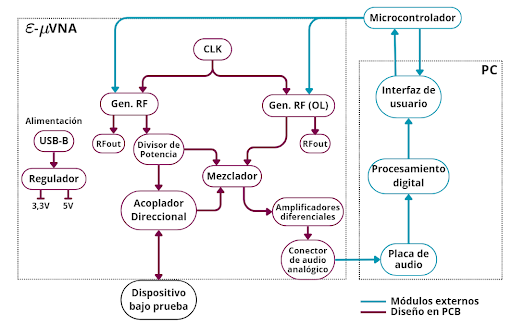
\includegraphics[width=0.8\linewidth]{Imagenes/diagbloques.png}
    \caption{Diagrama en bloques del sistema}
    \label{fig:diagbloques}
\end{figure}

A continuación, se detalla la solución del hardware, software, firmware e interfaz de usuario.

\section{Hardware}
El hardware se diseñó en su totalidad en el software Altium Designer, con una licencia estudiantil gracias al programa Altium Student Lab \cite{altium_designer}. Se creó una librería con los esquemáticos, footprints y modelos 3D de los componentes a utilizar. Se dividió el proyecto en esquemáticos que representan los distintos bloques funcionales. En principio se planteó un modelo de 2 capas, con FR4 como dieléctrico de 0,8 mm de espesor.  

\section{Firmware}
El firmware se programó en lenguaje C++ en el entorno Arduino IDE. 

\section{Software}

\section{Interfaz de usuario}
La interfaz de usuario se programó con PyQt6, mediante un prompt de la inteligencia artificial (IA) Claude, modelo Sonnet 5 Esfuerzo Medio. Se alimentó del software original, que tenía la lógica de medición funcionando, pero que corría secuencialmente y se comunicaba con el usuario a través de la consola. 

El prompt inicial fue: "Quiero hacer una interfaz de usuario sencilla que me permita comunicarme con este script. que se pueda elegir frecuencias y paso, visualizar modulo y fase de S11 y abaco de smith, que permita hacer calibración. Qué plataforma/lenguaje recomendas, y cuanto tiempo tardaría en ponerla en funcionamiento?". La IA recomendó Python + PyQt6/PySide6, con matplotlib embebido para los gráficos. Dió las razones (reutilizar funciones, permite actualizar el plot en vivo, aprovecha librerías de Python para graficar) y explicó otras alternativas y por qué las descartó. Preguntó si hacía un esqueleto de la app con ventana principal, campos de frecuencia, threading de barrido y gráficos, y se le dió el permiso. Creó dos archivos, un "core" que contiene la misma lógica de cálculo que el código original pero reorganizada en funciones independientes (comunicación serial con Arduino, capura de audio, procesamiento de señal, detección del tono de batido y cálculo de S11 y álgebra de calibración) y un "GUI" (Graphical User Interface) que contiene la parte visual: ventana, botones, campos y gráficos. Este llama a las funciones implementadas en el core.

Se agregó la biblioteca PyQt6 para usar ventanas, botones, campos e hilos de ejecución. Se creó una clase (SweepWorker(QThread)) que se encarga de correr el barrido en segundo plano y avisar a la ventana qué se midió para que actualice los gráficos y la barra de progreso sin congelarse entre cada medición. 

La IA generó además el diagrama de flujo que se observa en la figura \ref{fig:d_flujo_interfaz}. Los códigos se encuentran en el capítulo "Esquemáticos y código" \ref{VNA_core}. 

\begin{figure}
    \centering
    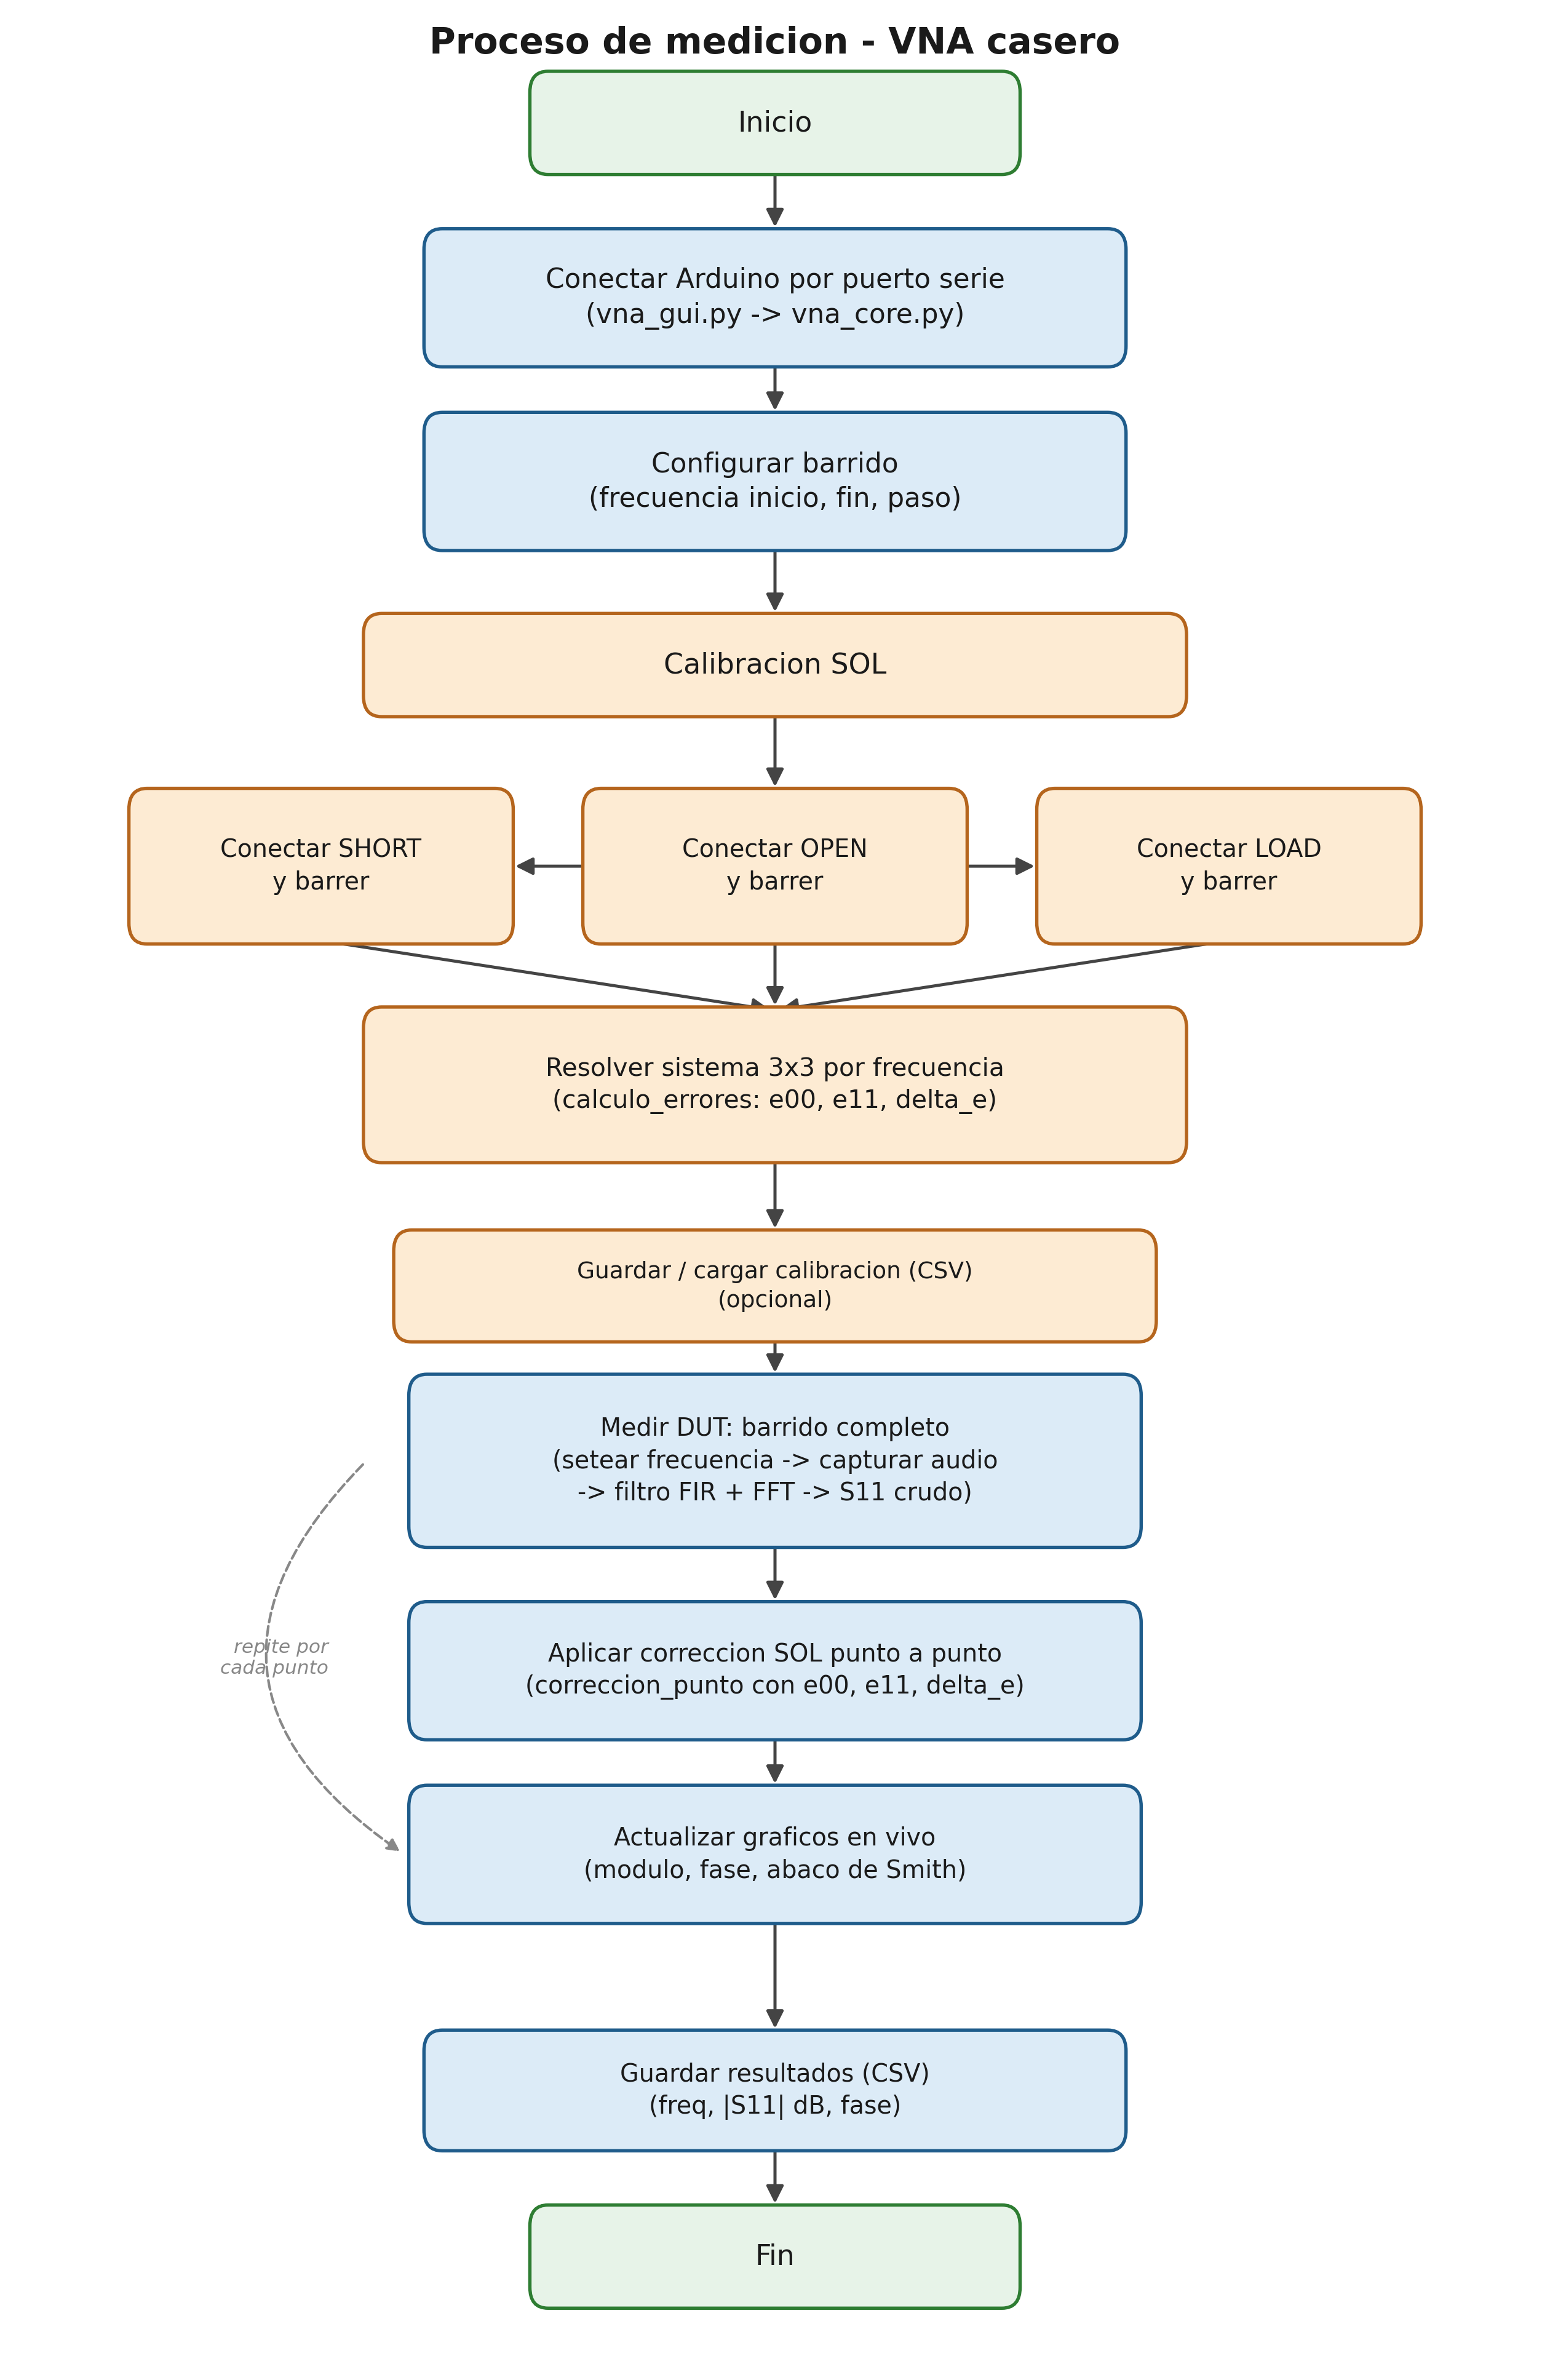
\includegraphics[width=0.5\linewidth]{Imagenes/d_flujo_interfaz.png}
    \caption{Diagrama de flujo de la interfaz de usuario}
    \label{fig:d_flujo_interfaz}
\end{figure}
